\documentclass[aspectratio=169]{beamer}
\usepackage{hyperref}
\usepackage[T1]{fontenc}
\usepackage{tikz}
\usepackage{xcolor}
\usepackage[french]{babel}
% A SISU beamer based on THU beamer.

% other packages
\usepackage{latexsym,amsmath,xcolor,multicol,booktabs,calligra}
\usepackage{graphicx,pstricks,listings,stackengine}
\renewcommand{\figurename}{Figure.}
\renewcommand{\tablename}{Table.}

\definecolor{appbg}{HTML}{f0f0f0}
\definecolor{chatbg}{HTML}{ffffff}
\definecolor{headerbg}{HTML}{4CAF50}
\definecolor{inputbg}{HTML}{e0e0e0}
\definecolor{sendbtn}{HTML}{4CAF50}
\definecolor{navbarbg}{HTML}{333333}
\definecolor{navbartext}{HTML}{ffffff}
\definecolor{windowborder}{HTML}{999999}

\author{Adil ABBADI , Abdelhak MEKAOUI}
\title{Conception, Développement et Déploiement d'un Chatbot Intelligent et d'une Plateforme E-Learning}
\institute{ENSA Agadir}
\date{\today}
\usepackage{sisu}

% defs
\def\cmd#1{\texttt{\color{red}\footnotesize $\backslash$#1}}
\def\env#1{\texttt{\color{blue}\footnotesize #1}}
\definecolor{deepblue}{rgb}{0,0,0.5}
\definecolor{deepred}{rgb}{0.6,0,0}
\definecolor{deepgreen}{rgb}{0,0.5,0}
\definecolor{halfgray}{gray}{0.55}

\lstset{
    basicstyle=\ttfamily\small,
    keywordstyle=\bfseries\color{deepblue},
    emphstyle=\ttfamily\color{deepred},    % Custom highlighting style
    stringstyle=\color{deepgreen},
    numbers=left,
    numberstyle=\small\color{halfgray},
    rulesepcolor=\color{red!20!green!20!blue!20},
    frame=shadowbox,
}


\begin{document}
\bibliographystyle{plain}
\bibliography{mybibfile}

\begin{frame}

  \begin{figure}[htpb]
        \begin{center}
         
\includegraphics[width=0.3\linewidth]{pic/logo.png}
         \hfill
            
\includegraphics[width=0.3\linewidth]{pic/code.png}
        \end{center}
    \end{figure}
    
    \titlepage



    \begin{tikzpicture}[remember picture, overlay]
        % Define the coordinates where you want the block to be placed
        \coordinate (block) at ([yshift=-8.3cm]current page.north);
    
        % Place the block at the defined coordinates
        \node[above, text width=\linewidth, text=black,fill = white] at (block) {
            \begin{minipage}{\linewidth}
                \centering
                \begin{minipage}[t]{0.45\linewidth}
                    \begin{center}
                        \small
                        \textbf{Jury:} \\
                        M. A EL YOUSFI \\
                        M. H AKSASSE \\
                        M. M ELYAAKOUBI \\
                        


                        % Ajoutez d'autres membres du jury si nécessaire
                    \end{center}
                \end{minipage}
                \hfill
                \begin{minipage}[t]{0.45\linewidth}
                    \begin{center}
                        \small
                        \textbf{Encadré par:} \\
                        M. A EL YOUSFI\\
                        M. H Elkina\\
                        

                        % Ajoutez d'autres encadrants si nécessaire
                    \end{center}
                \end{minipage}
            \end{minipage}
        };
    \end{tikzpicture}
  
\end{frame}


\begin{frame}
    \tableofcontents[sectionstyle=show,subsectionstyle=show/shaded/hide,subsubsectionstyle=show/shaded/hide]
\end{frame}

\section{Introduction}

\subsection{Contexte general}


\begin{frame}{Organisme d'accueil}
 
    \vspace{0.5cm} % Adjust space between image and text
    \begin{block}{\centering \textbf{\Large Le centre Code 212}}
        \centering
        \vspace{0.2cm} % Adjust space within the block
        Le Code 212, lancé dans le cadre du PACTE ESRI-2030 au Maroc, est un centre de formation et de certification dédié aux métiers du digital, visant à renforcer les compétences numériques et à promouvoir l’innovation pour répondre aux besoins du marché.
    \end{block}

\begin{figure}[htpb]
    \centering
      \begin{minipage}[b]{0.45\linewidth}
        \centering
        
\includegraphics[width=\linewidth]{pic/esri.png}
    \end{minipage}
    \begin{minipage}[b]{0.45\linewidth}
        \centering
        
\includegraphics[width=\linewidth]{pic/code.png}
    \end{minipage}
\end{figure}
\end{frame}


\begin{frame}{Centre Code212 : Ses Fonctionnalités et Services}
 
   \begin{figure}[htpb]
    \centering
      \begin{minipage}[b]{0.45\linewidth}
        \centering
        
\includegraphics[width=\linewidth]{pic/formation.jpg}
    \end{minipage}
    \begin{minipage}[b]{0.45\linewidth}
        \centering
        
\includegraphics[width=\linewidth]{pic/certificat.png}
    \end{minipage}
\end{figure}
\end{frame}



\subsection{Problematique}
\begin{frame}{Problematique}
\begin{figure}[htpb]
        \centering
        
\includegraphics[height=3cm]{pic/question.png}
    \end{figure}
  Face à la diversité des services offertes par Code 212 et l'université UIZ en général, les étudiants sont confrontés à une multitude de questions en temps réel. Quelle solution technologique peut répondre efficacement à ce besoin en fournissant un guide instantané et personnalisé ?
\end{frame}

\subsection{Solution proposee}
\begin{frame}{Solution proposee}

Le chatbot IA de Code 212 offre une assistance instantanée aux étudiants en temps réel, optimisant ainsi les ressources pédagogiques du centre.
\begin{figure}[htpb]
        \centering
        
\includegraphics[height=3cm]{pic/ia.png}
    \end{figure}
\end{frame}

\begin{frame}{Un Chatbot Inspiré par ChatGPT}

S'inspirant de ChatGPT, un outil de réponse automatisée, une solution similaire pourrait efficacement répondre aux besoins de recherche des utilisateurs, en fournissant des informations pertinentes en temps réel pour faciliter l'accès et le traitement des connaissances.

\begin{figure}[htpb]
        \centering
        
\includegraphics[height=3cm]{pic/chatgpt.png}
    \end{figure}
\end{frame}

\subsection{Fonctionnalités attendues}


\begin{frame}{Fonctionnalités Axées sur l'Utilisateur}
    \begin{figure}[htpb]
        \centering
        
\includegraphics[height=3cm]{pic/user.png}
    \end{figure}
\begin{itemize}
    \setlength\itemsep{0.8em} % Adjust the spacing between items
     \item \textbf{Interaction avec chatbot}
    \item \textbf{Inscription à un cours}
    \item \textbf{Inscription à un événement}
    \item \textbf{Demande de certificat} 

\end{itemize}

\end{frame}


\begin{frame}{Fonctionnalités Axées sur l'administrateur}
    \begin{figure}[htpb]
        \centering
        
\includegraphics[height=3cm]{pic/admin.png}
    \end{figure}

    \begin{itemize}
        \setlength\itemsep{0.8em} % Adjust the spacing between items
     
        \item \textbf{Gestion des cours}
        \item \textbf{Gestion des événements}
        \item \textbf{Gestion des certificats}
        \item \textbf{Gestion des utilisateurs}
    \end{itemize}
    
    \end{frame}





\section{Analyse et Conception du Project}
\subsection{Analyse du besoin}
\begin{frame}{Analyse du besoin}
\begin{figure}[htpb]
        \centering
        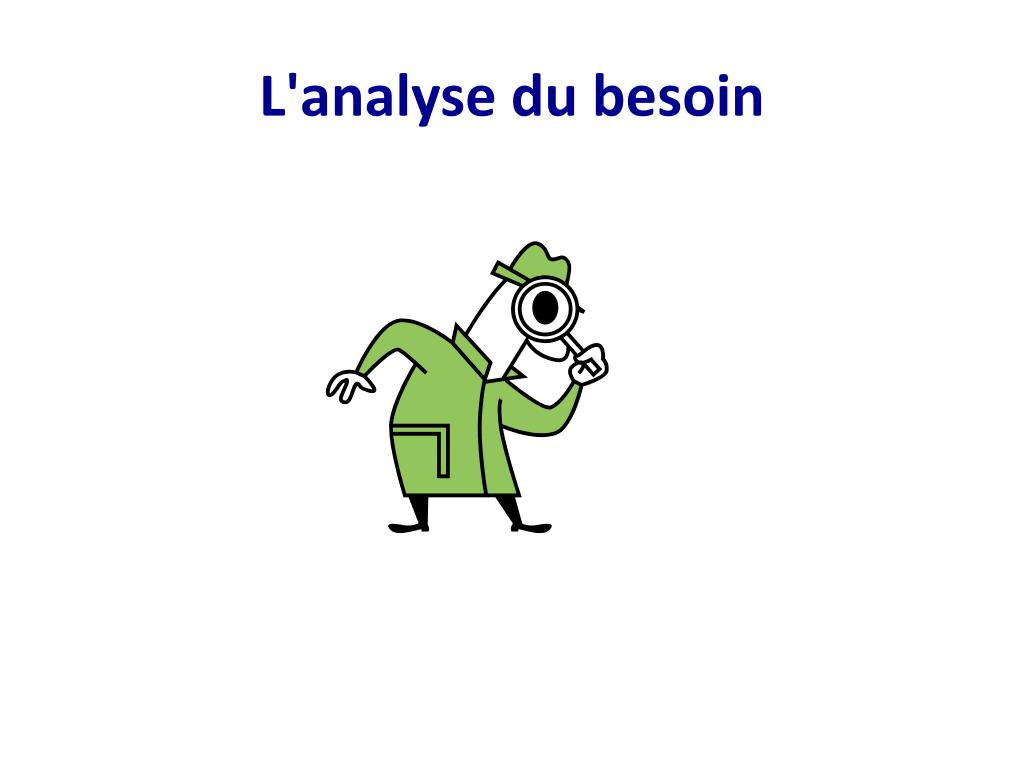
\includegraphics[height=5cm]{pic/analyse-besoin.jpg}
    \end{figure}

\end{frame}

\subsection{Digramme cas d'utilisation}
\begin{frame}{Digramme cas d'utilisation}
 \begin{figure}[htpb]
        \centering
        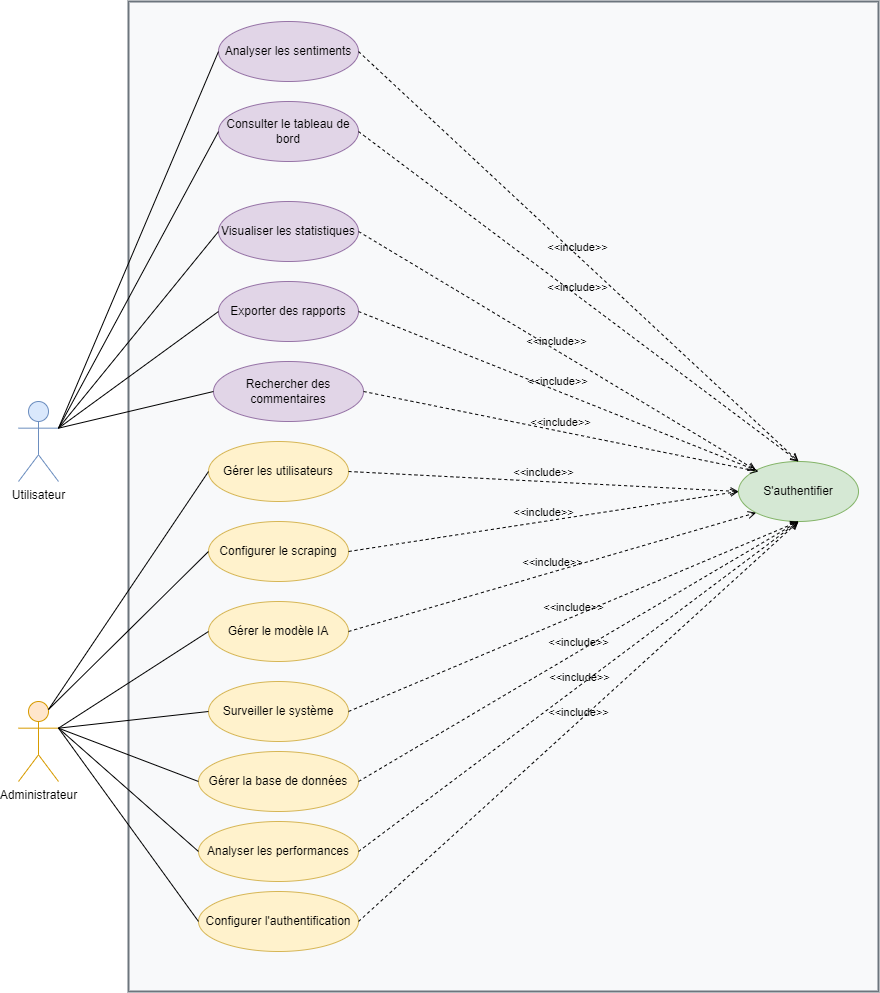
\includegraphics[height=7.5cm]{pic/usecase.png}
    \end{figure}
\end{frame}


\subsection{Methodology}
\begin{frame}{Methodology}
    
    \begin{figure}[htpb]
        \centering
        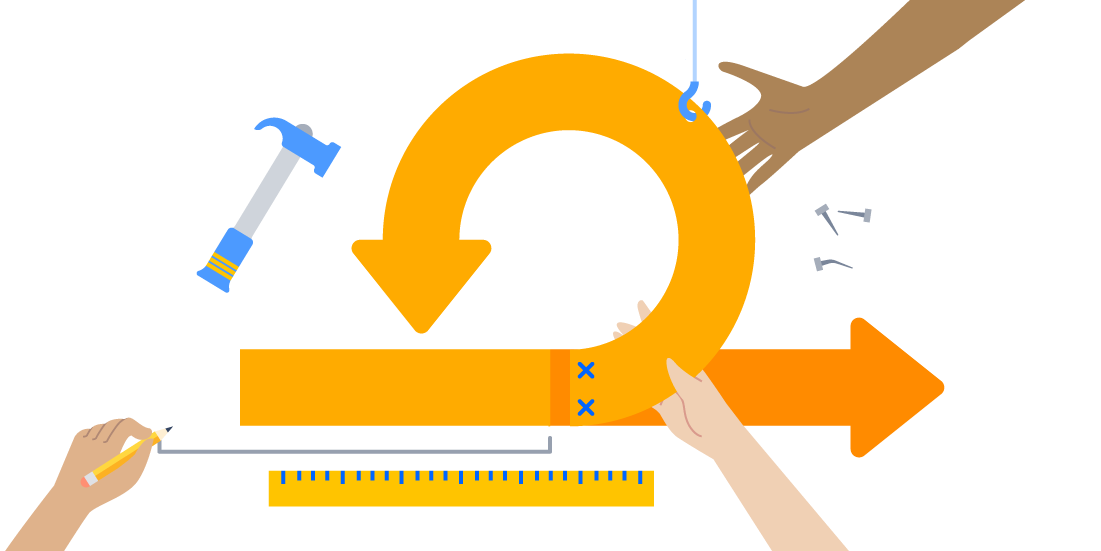
\includegraphics[height=4cm]{pic/scrum.png}
    \end{figure}

    Afin de gérer au mieux ce projet, nous avons opté pour la méthode SCRUM et divisé les différents modules en sprints.
\end{frame}


\subsection{Planification}
\begin{frame}{Planification}
 
 \begin{figure}[htpb]
        \centering
        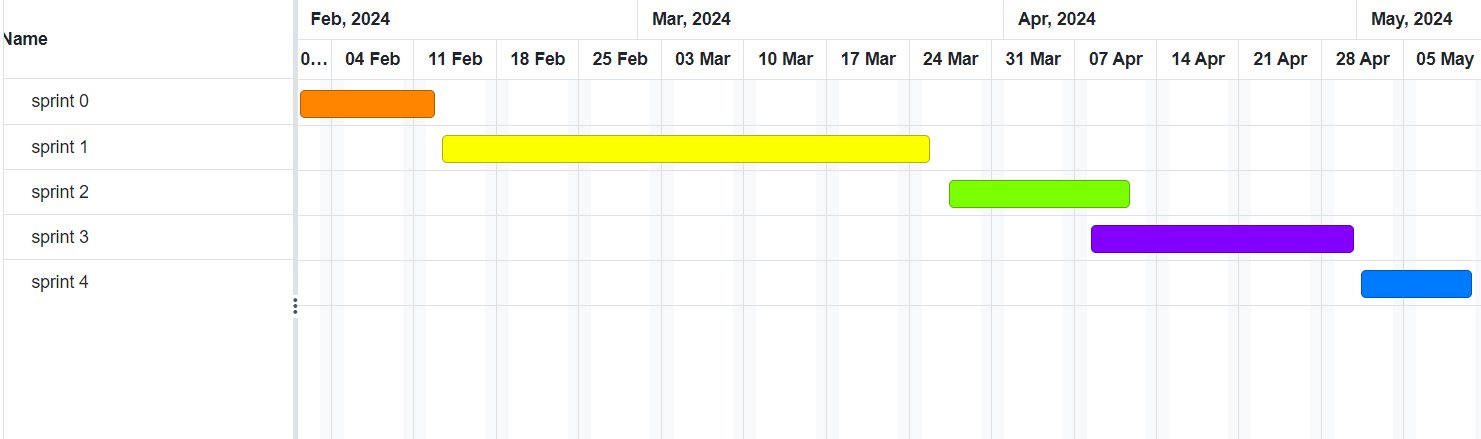
\includegraphics[height=3.5cm]{pic/gant-prev.png}
    \end{figure}
\end{frame}


\subsection{Prototype}
\begin{frame}{Prototype}

 \begin{figure}[htpb]
        \centering
        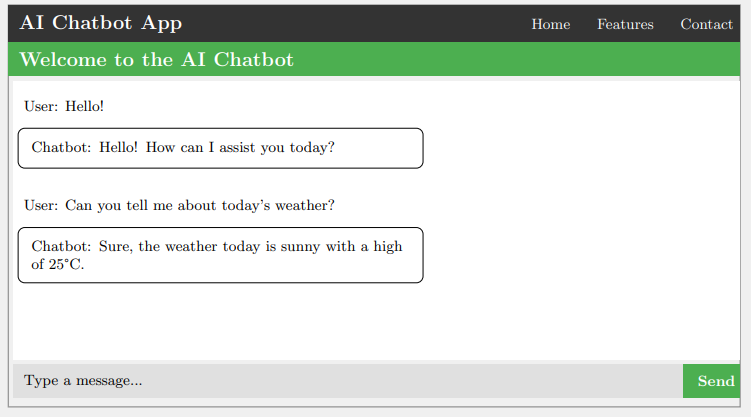
\includegraphics[height=6cm]{pic/prototype.png}
    \end{figure}
    
\end{frame}


\section{Spécifications Techniques}



\subsection{Architecture microsevice}



\begin{frame}{Architecture microservice}
   \begin{figure}[htpb]
        \centering
        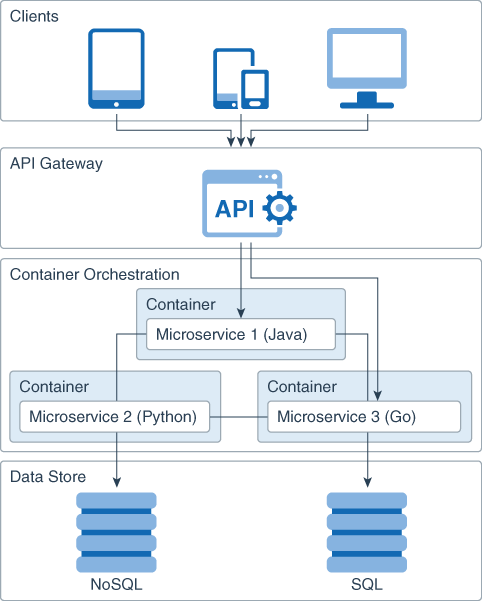
\includegraphics[height=7cm]{pic/microservice_architecture_presentation.png}
    \end{figure}
\end{frame}


\begin{frame}{Architectures prévues}
    \begin{figure}[htpb]
         \centering
         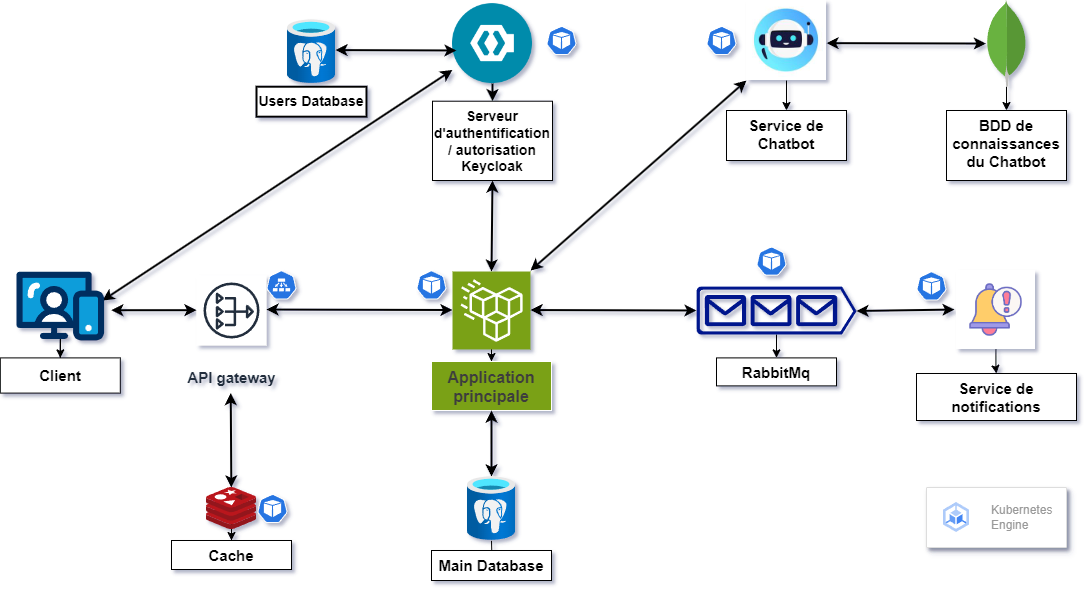
\includegraphics[height=5cm]{pic/Code212_architecture.drawio (1).png}
     \end{figure}
 \end{frame}


\subsection{Benchmark}
\begin{frame}{Benchmark Backend}
   \begin{figure}[htpb]
        \centering
        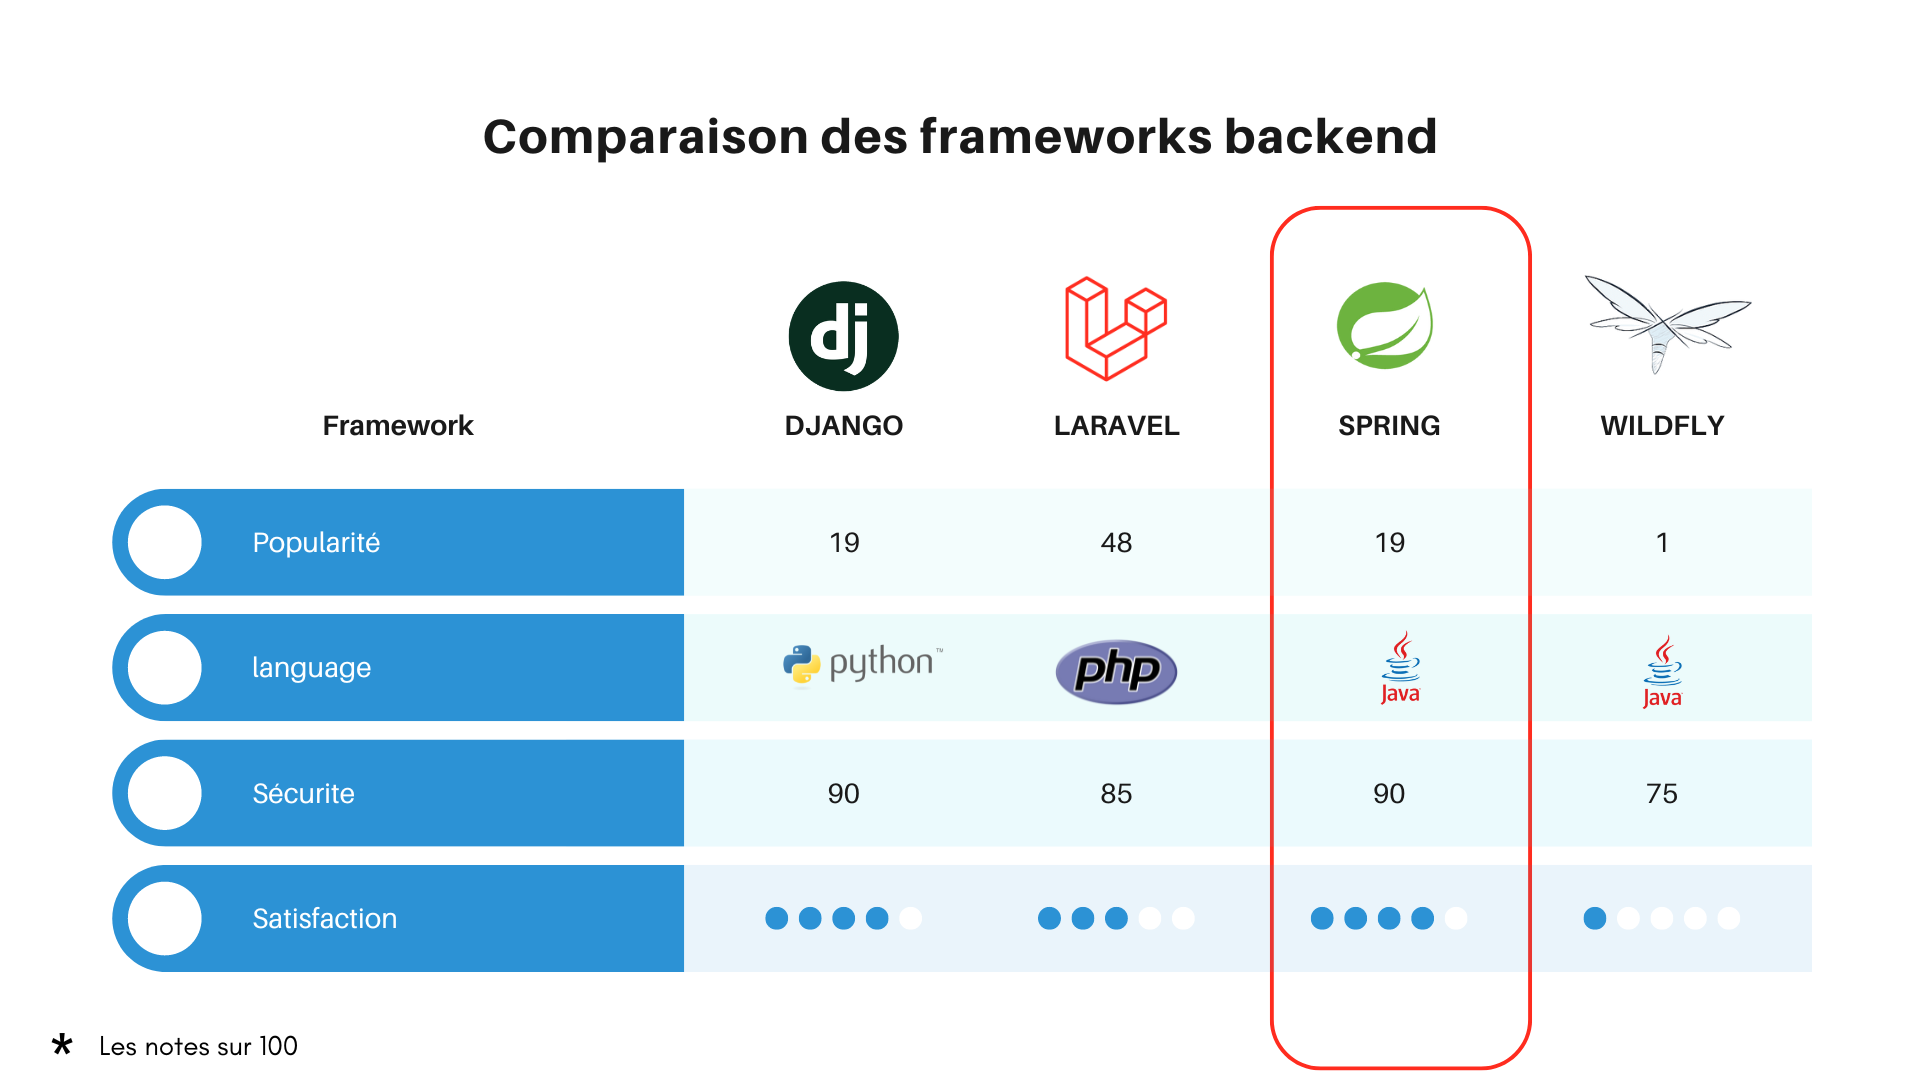
\includegraphics[height=5cm]{pic/benchmark.png}
    \end{figure}
\end{frame}

\begin{frame}{Benchmark Fronted}
    \begin{figure}[htpb]
         \centering
         
\includegraphics[height=5cm]{pic/bench-next.jpg}
     \end{figure}
 \end{frame}

 \begin{frame}{Benchmark model IA}
    \begin{figure}[htpb]
         \centering
         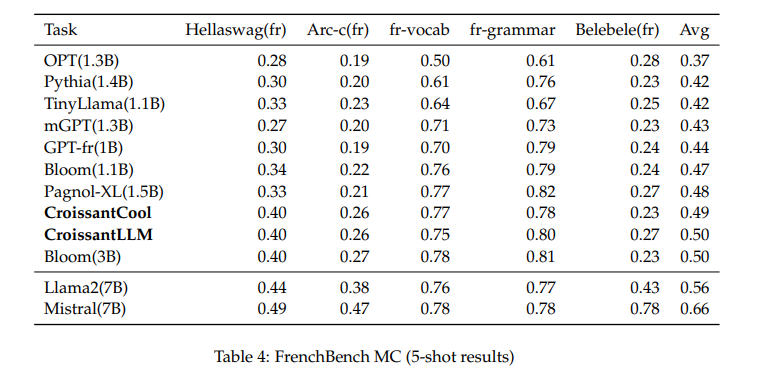
\includegraphics[height=6cm]{pic/ia_benchmark.png}
     \end{figure}
 \end{frame}

\subsection{Technologies Sélectionnées}
\begin{frame}{Technologies choisies pour les services}
    \begin{figure}[htpb]
        \centering
        \begin{minipage}{0.32\textwidth}
            \centering
            
\includegraphics[height=3cm]{pic/next.png}
        \end{minipage}%
        \hspace{0.03\textwidth}
        \begin{minipage}{0.32\textwidth}
            \centering
            
\includegraphics[height=3cm]{pic/spring.png}
        \end{minipage}%
        \hspace{0.03\textwidth}
        \begin{minipage}{0.32\textwidth}
            \centering
            
\includegraphics[height=3cm]{pic/keycloak.png}
        \end{minipage}
        
    \end{figure}
\end{frame}



\begin{frame}{Technologies choisies pour IA}
    \begin{figure}[htpb]
        \centering
       
        \begin{minipage}{0.5\textwidth}
            \centering
            
\includegraphics[height=2cm]{pic/tinyllama.png}
        \end{minipage}
        \hspace{0.1\textwidth}
        \begin{minipage}{0.5\textwidth}
            \centering
            
\includegraphics[height=2cm]{pic/langchain.jpeg}
        \end{minipage}
        \hspace{0.1\textwidth}
        \begin{minipage}{0.5\textwidth}
            \centering
            
\includegraphics[height=2cm]{pic/mongo.png}
        \end{minipage}
    \end{figure}
\end{frame}

\subsection{Communication entre services}
\begin{frame}{Communication entre services}
   \begin{figure}[htpb]
        \centering
        
\includegraphics[height=2cm]{pic/rest.png}
         \hspace{0.1\textwidth}
         
\includegraphics[height=2cm]{pic/kafka.png}
    \end{figure}
\end{frame}

\subsection{Conclusion}
\begin{frame}{Conclusion}

    Cette étude technique détaille l'architecture des microservices, les technologies utilisées, et les interactions entre les services, garantissant une application modulaire, sécurisée, et scalable avec Keycloak pour la gestion des identités et des accès. Les choix de conception visent à assurer une expérience utilisateur optimale tout en garantissant performance et sécurité.
\end{frame}

\section{Realisation et mise en oeuvre}


\subsection{Sprints}
\begin{frame}{Sprints reels (1)}
 
    \begin{figure}[htpb]
           \centering
           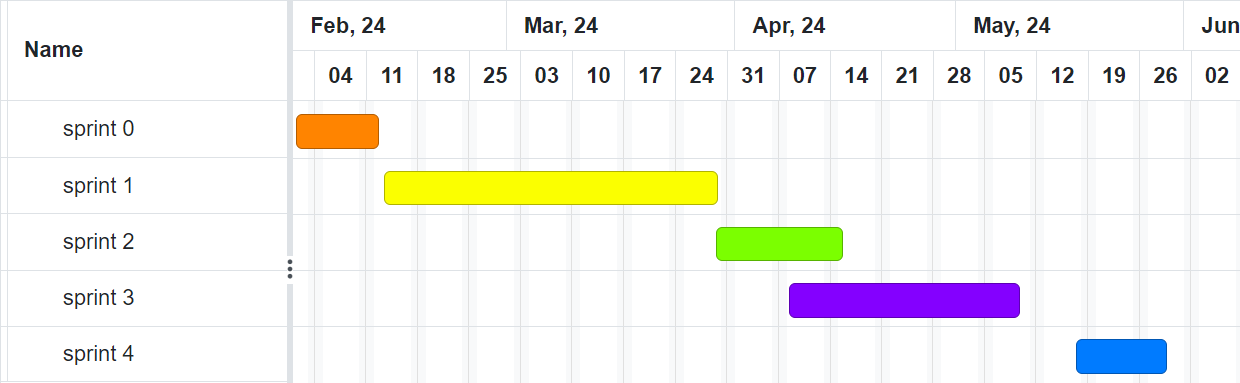
\includegraphics[height=3.5cm]{pic/gantt-reel.png}
       \end{figure}
   \end{frame}

   \begin{frame}{Sprints reels (2)}
 
    \begin{itemize}
        \item Sprint 1:
        \begin{itemize}
            \item Planification et configuration initiale du chatbot (User Story 1.1)
            \item Base de connaissances du chatbot (User Story 1.2)
        \end{itemize}
        
        \item Sprint 2:
        \begin{itemize}
            \item Mise à jour de la base de données par l’administrateur (User Story 1.3)
            \item Consultation des cours disponibles (User Story 2.1)
        \end{itemize}
        
        \item Sprint 3:
        \begin{itemize}
            \item Inscription aux cours et événements (User Story 2.2)
            \item Inscription aux examens de certification gratuits (User Story 2.3)
        \end{itemize}
        
        \item Sprint 4:
        \begin{itemize}
            \item Amélioration de l’interface utilisateur (User Story 3.1)
            \item Optimisation des performances du chatbot, déploiement et création des conteneurs (User Story 3.2)
        \end{itemize}
    \end{itemize}
    
   \end{frame}



\subsection{Sprint 1: D´eveloppement et D´eploiement du Chatbot}
\begin{frame}{Diagramme de cas d'utilisation}

\begin{figure}[htpb]
        \centering
        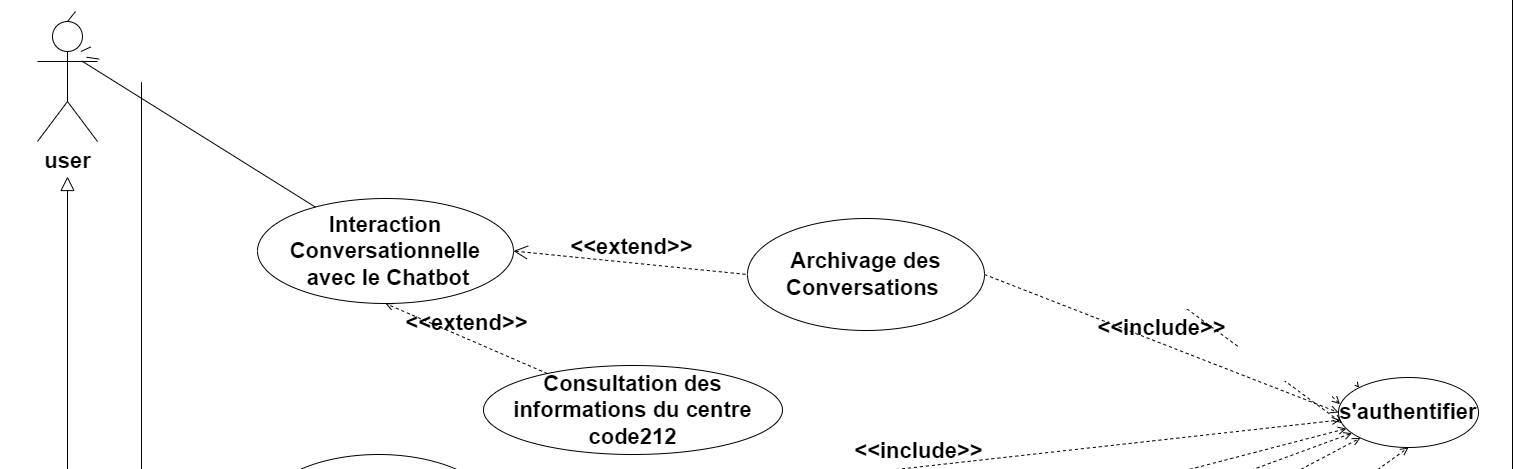
\includegraphics[height=5cm]{pic/sprint1-usecase.png}
\end{figure}
\end{frame}

\begin{frame}{Diagramme de classe}

\begin{figure}[htpb]
        \centering
        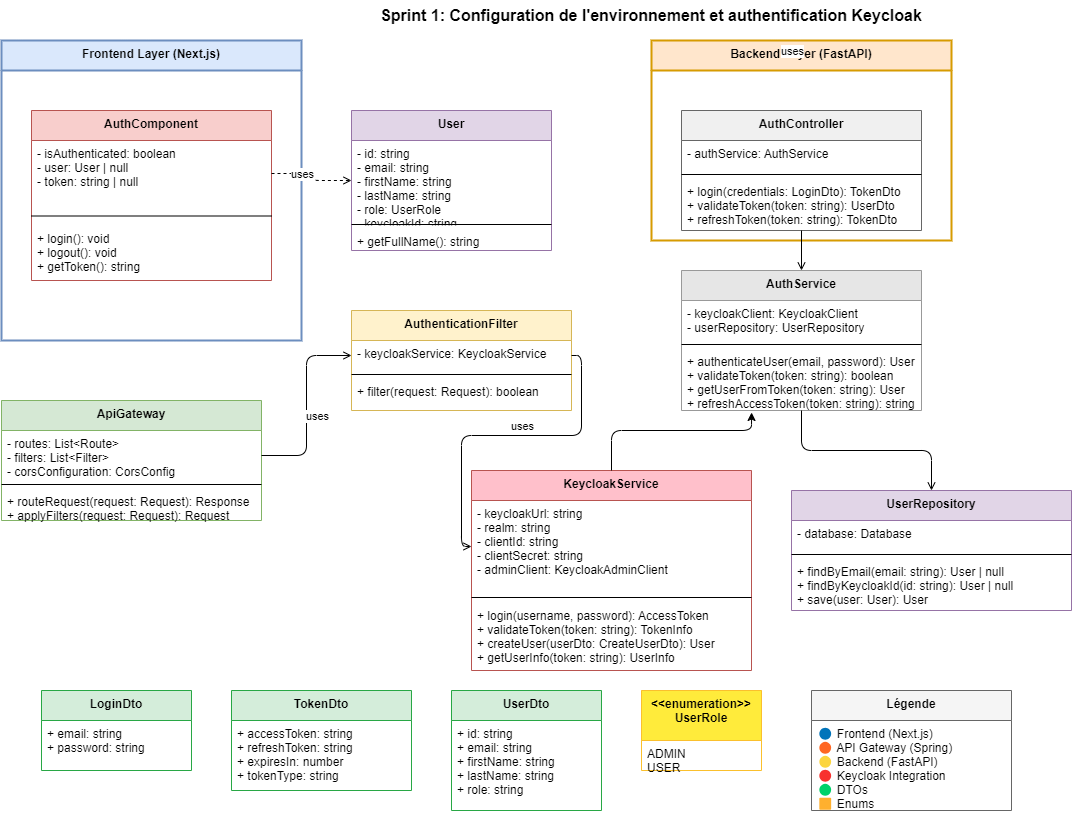
\includegraphics[height=5cm]{pic/sprint1-class.png}
\end{figure}
\end{frame}

\begin{frame}{Diagramme de sequence}
\begin{figure}[htpb]
        \centering
        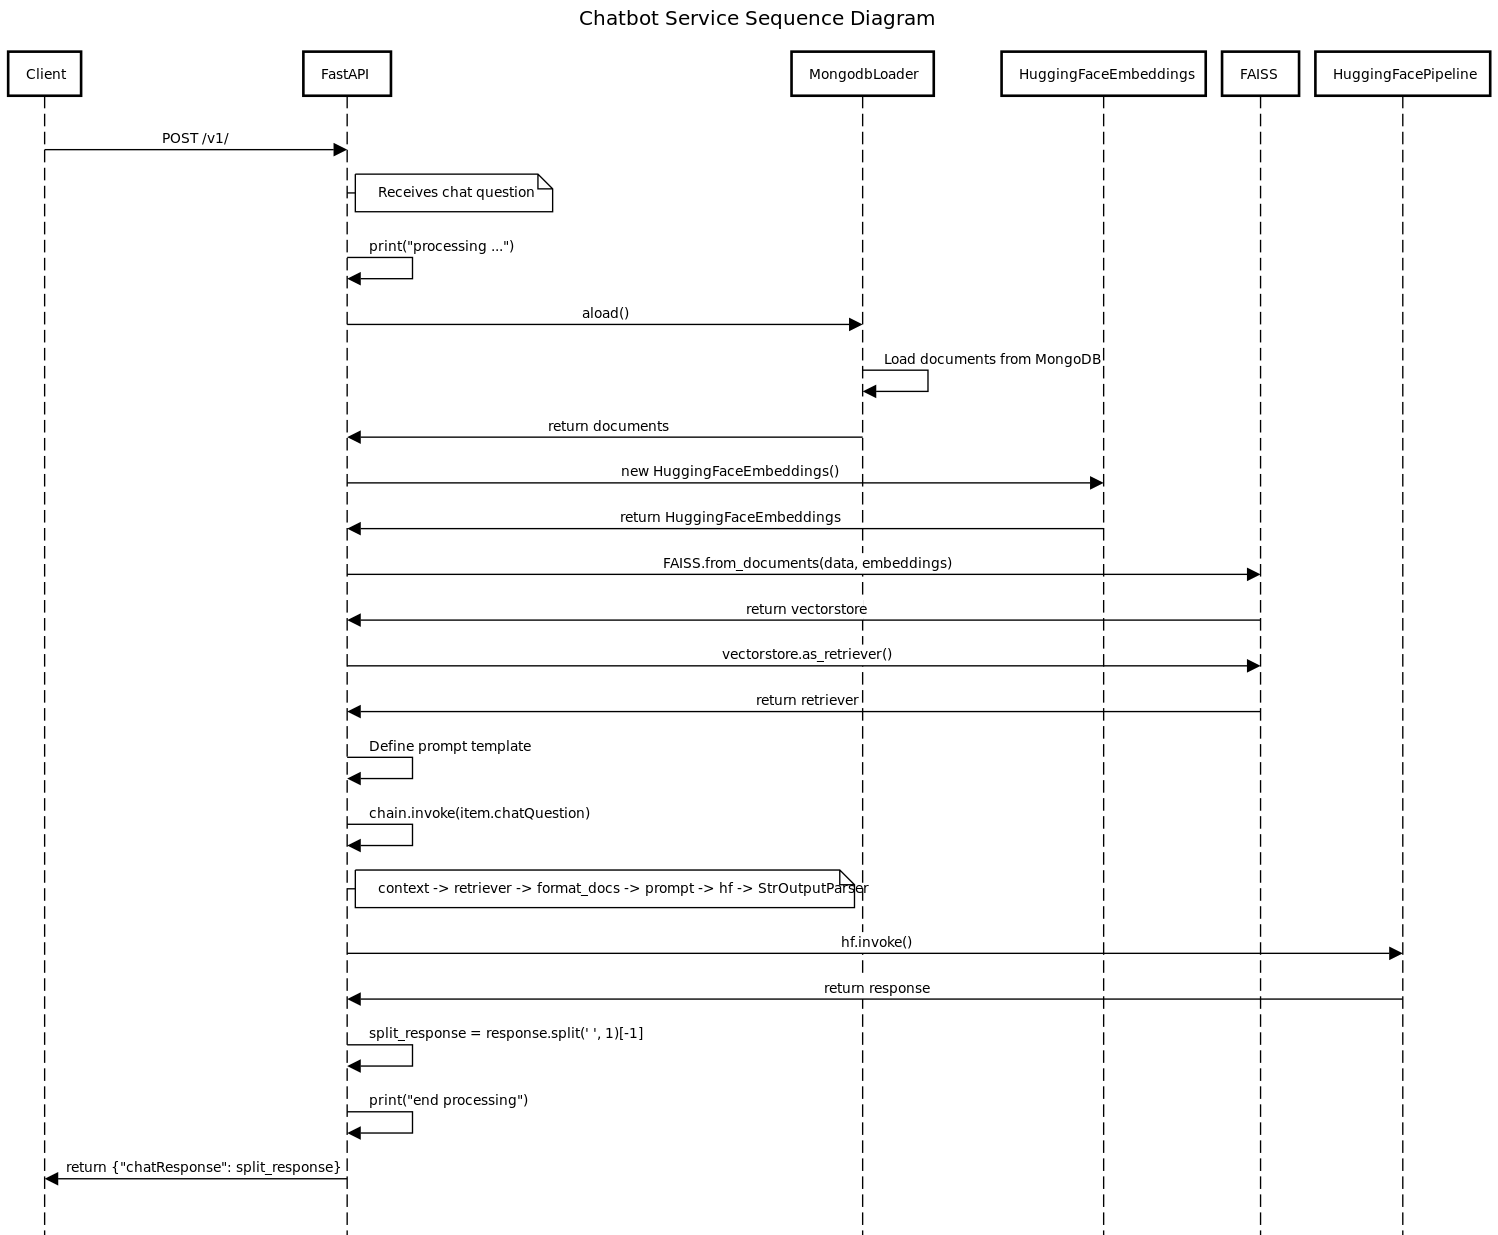
\includegraphics[height=8cm]{pic/chatbot-seq.png}
\end{figure}
\end{frame}

\begin{frame}{Realisation}
\begin{figure}[htpb]
        \centering
        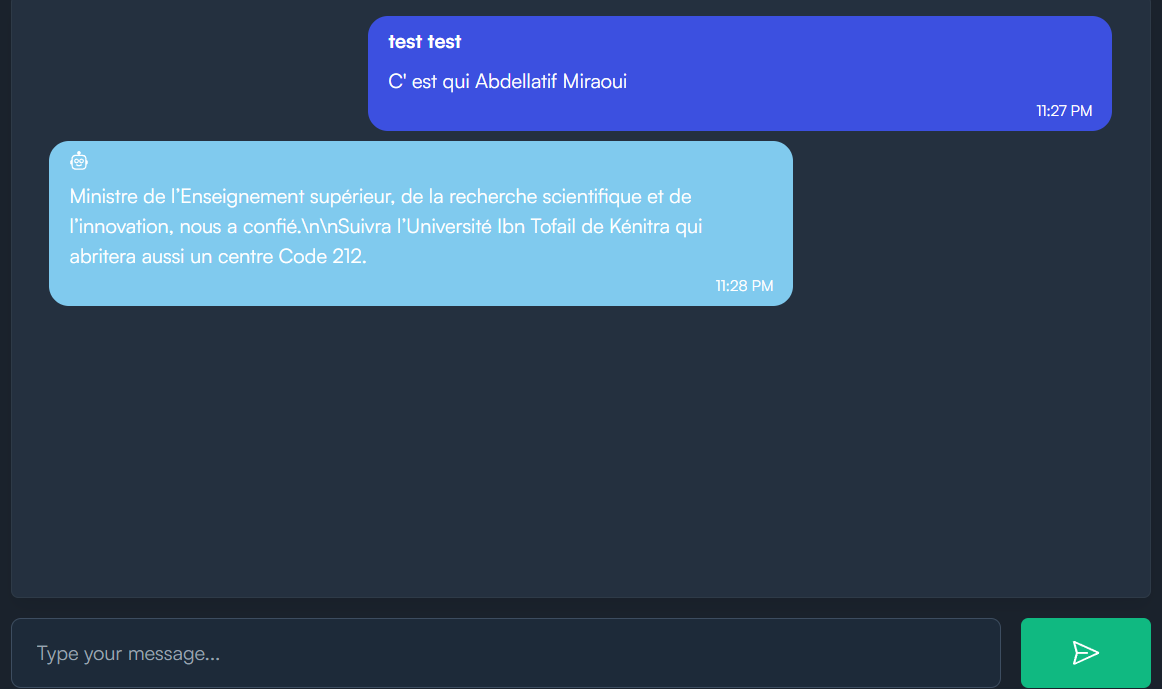
\includegraphics[height=6cm]{pic/chat2.png}
\end{figure}
\end{frame}

\subsection{Execution}
\begin{frame}{Execution}
    Demonstration de l'application
\end{frame}


\subsection{Sprint 2: Authentification et mise a jour de la
base de donnees par l’administrateur}
\begin{frame}{Diagramme de cas d'utilisation}

\begin{figure}[htpb]
        \centering
        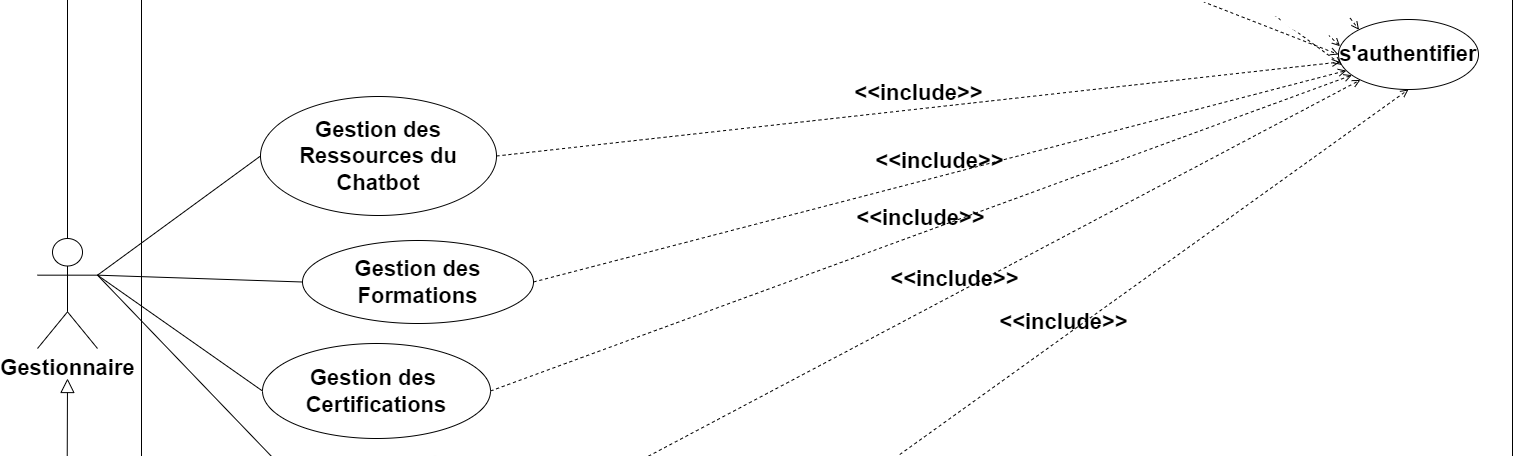
\includegraphics[height=5cm]{pic/sprint2-usecase.png}
\end{figure}
\end{frame}

\begin{frame}{Diagramme de classe}

\begin{figure}[htpb]
        \centering
        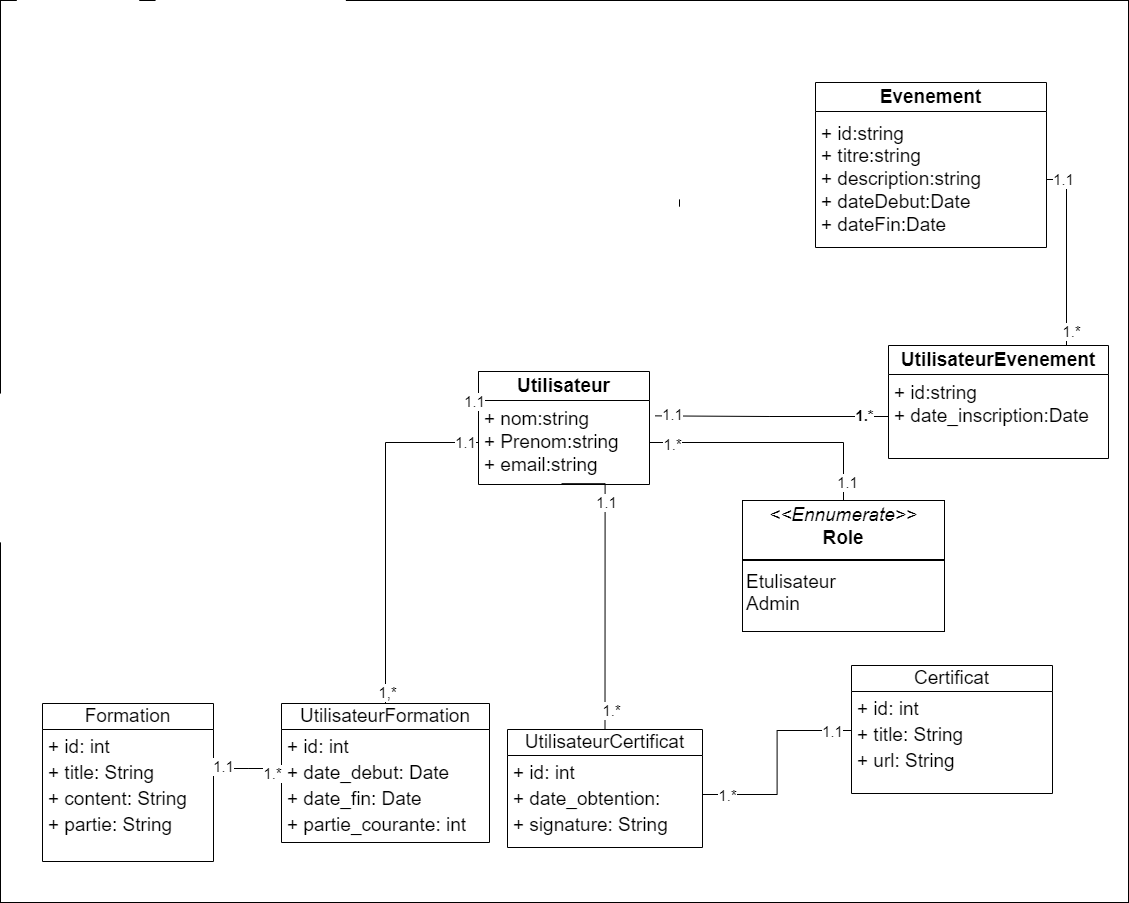
\includegraphics[height=5cm]{pic/sprint2-class.png}
\end{figure}
\end{frame}

\begin{frame}{Diagramme de sequence d'authentification}
\begin{figure}[htpb]
        \centering
        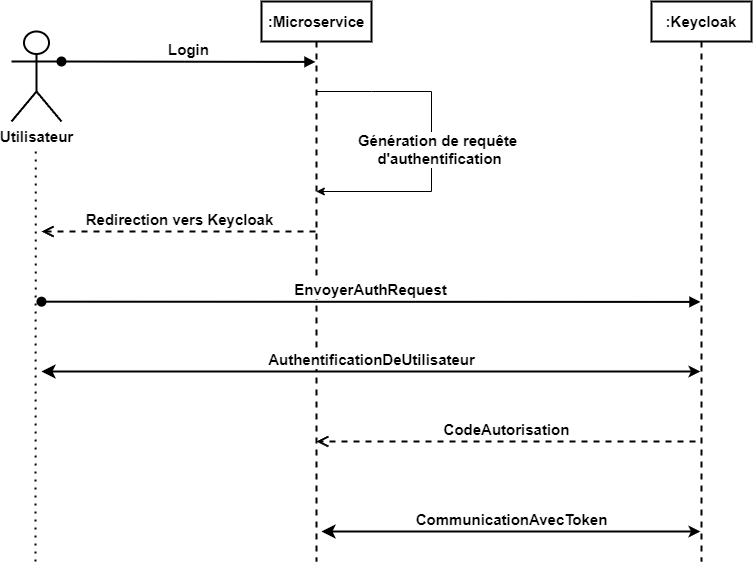
\includegraphics[height=8cm]{pic/keycloak-seq.png}
\end{figure}
\end{frame}

\begin{frame}{Diagramme de sequence de gestion des resources du chatbot}
\begin{figure}[htpb]
        \centering
        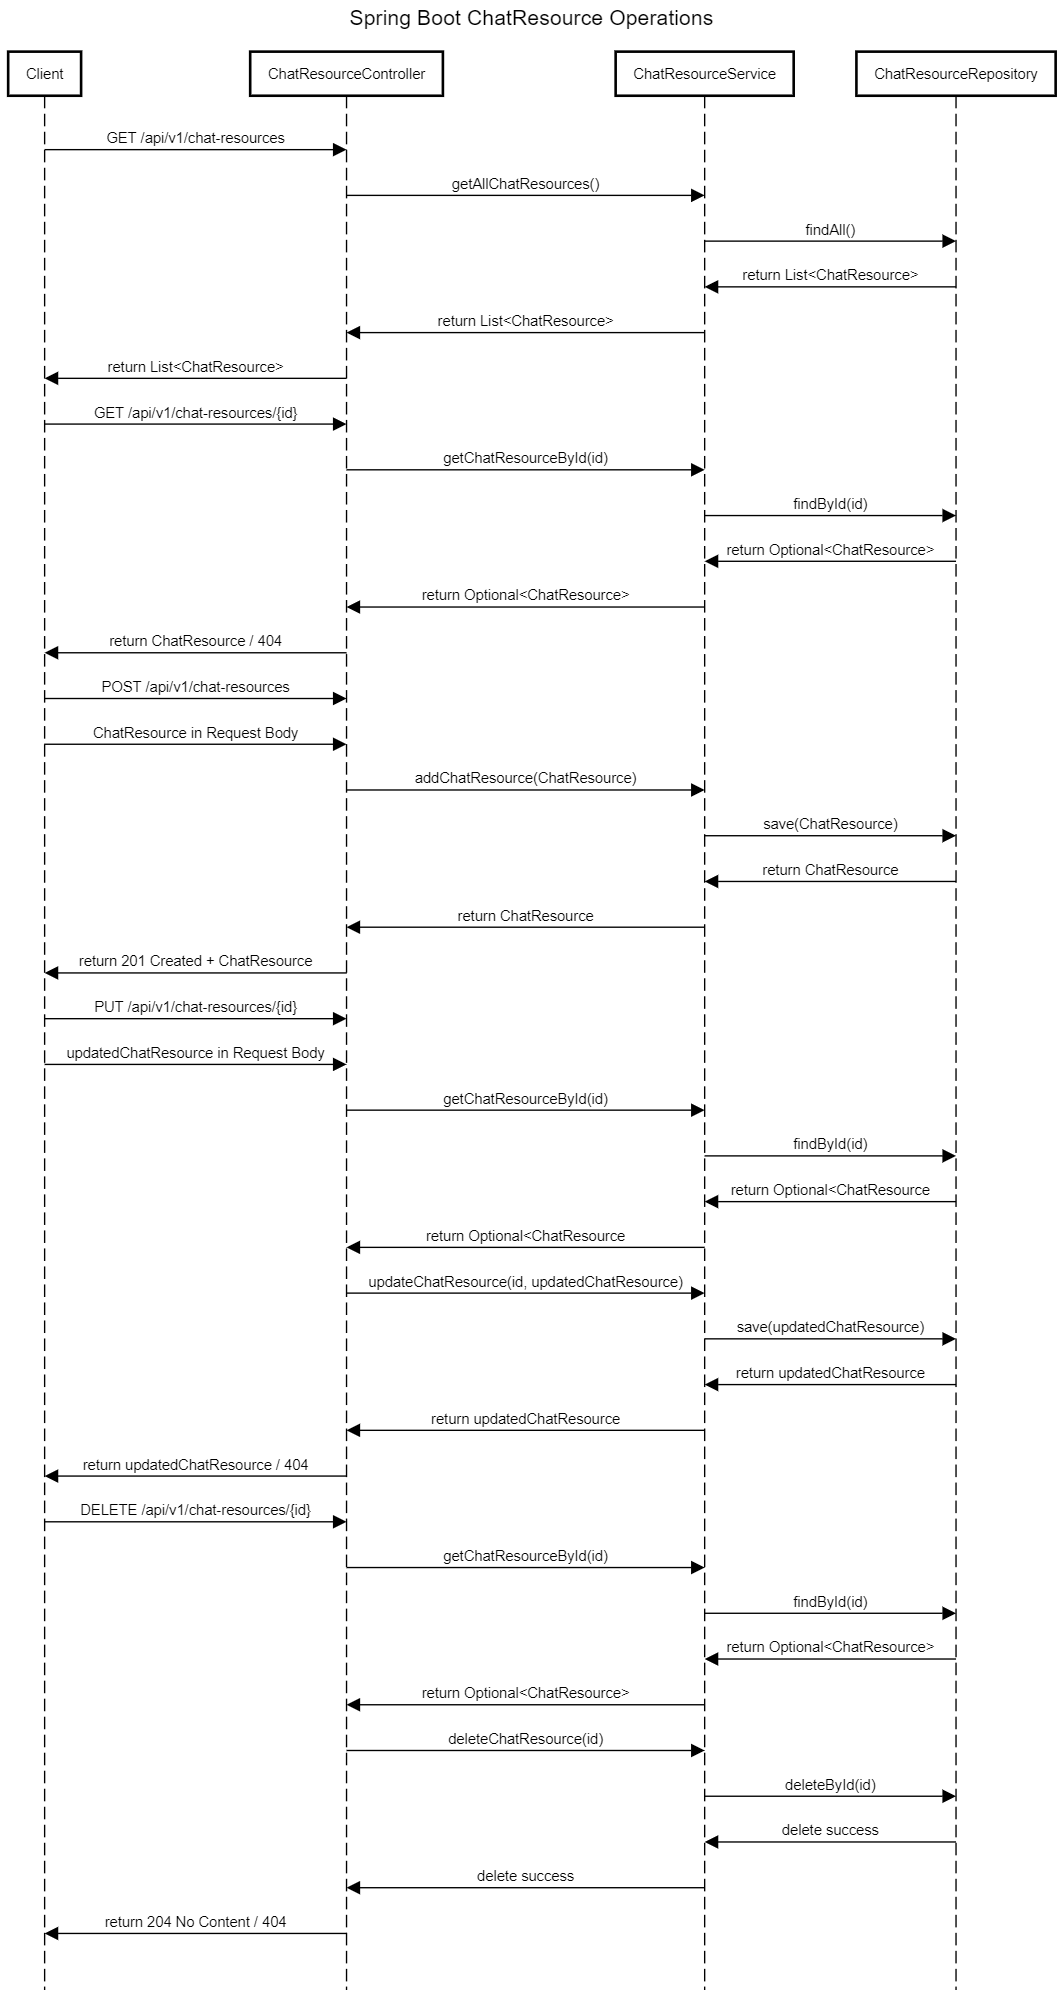
\includegraphics[height=8cm]{pic/chat-res-seq.png}
\end{figure}
\end{frame}

\begin{frame}{Realisation}
\begin{figure}[htpb]
        \centering
        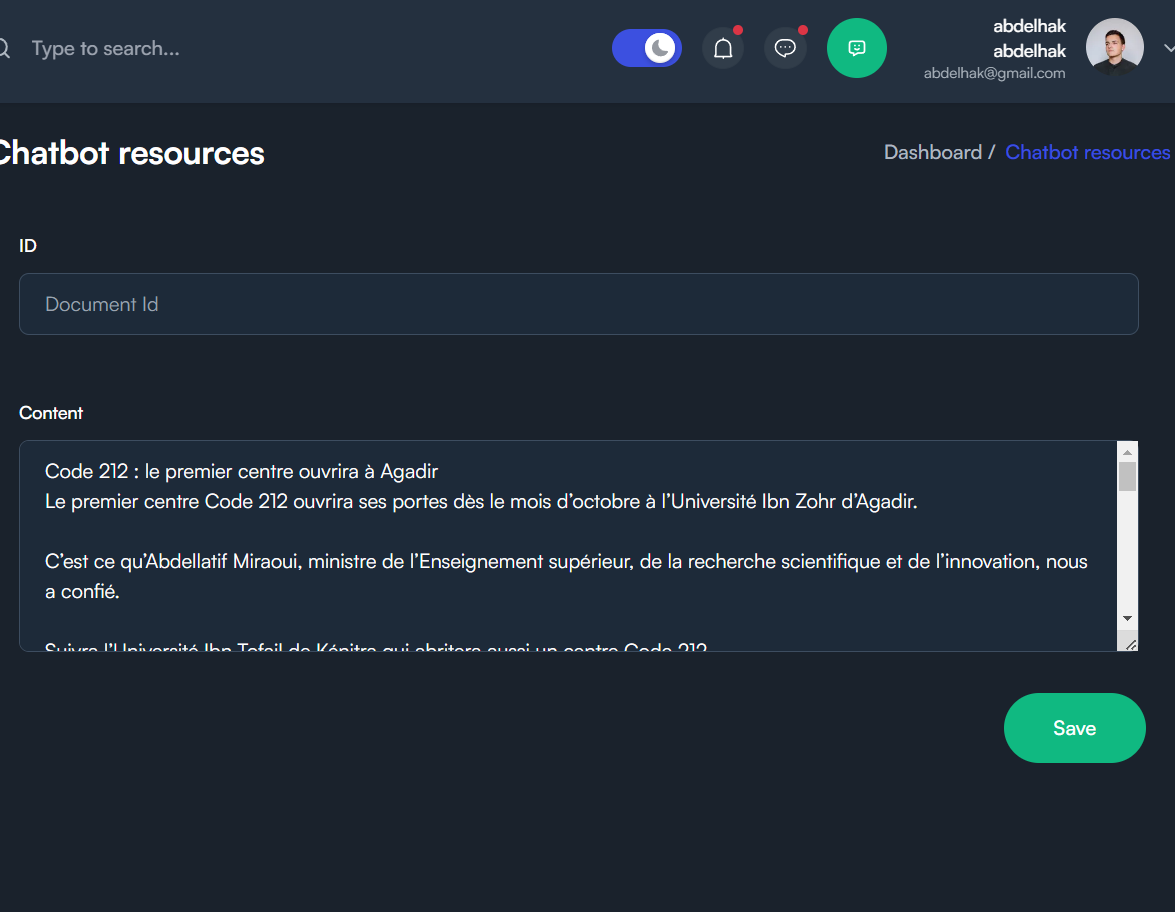
\includegraphics[height=6cm]{pic/admin-doc.png}
\end{figure}
\end{frame}

\subsection{Execution}
\begin{frame}{Execution}
    Demonstration de l'application
\end{frame}

\section{Conclusion}

\begin{frame}{Conclusion}
    \begin{figure}[htpb]
        \centering
        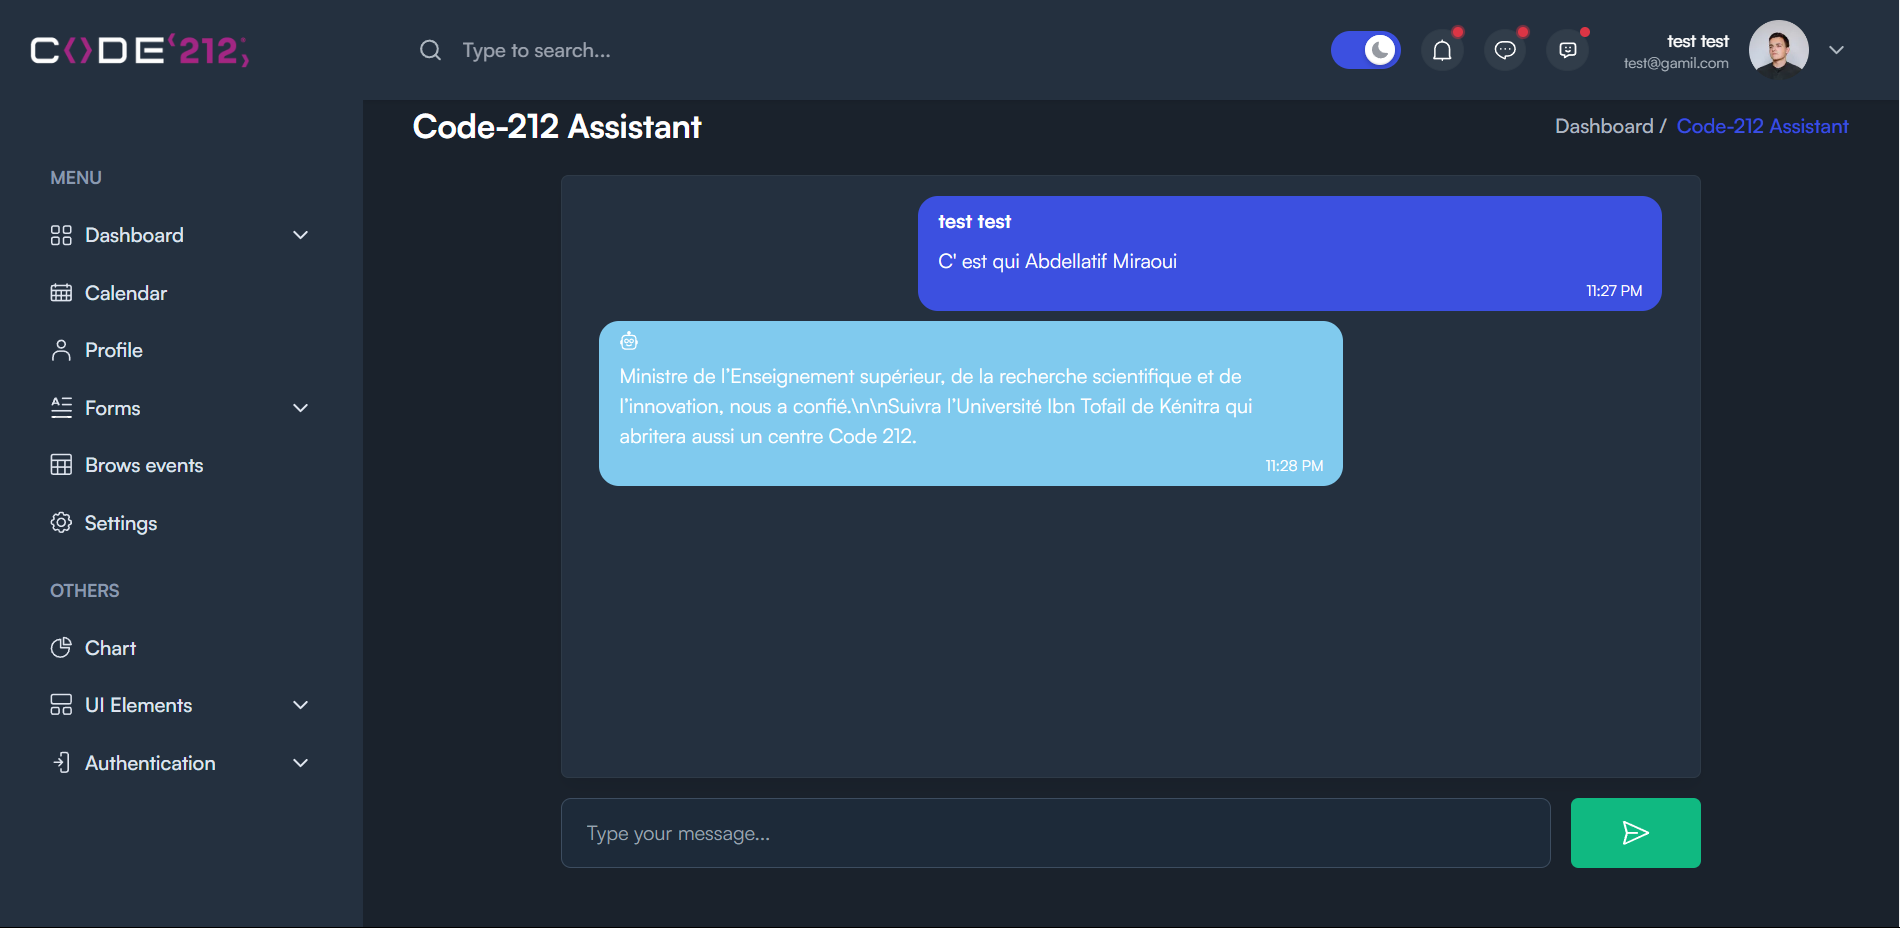
\includegraphics[height=5cm]{pic/chat1.png}
    \end{figure}
    En résumé, le projet vise à intégrer un chatbot AI dans une plateforme e-learning, offrant une expérience d’apprentissage améliorée pour les étudiants et une gestion efficace des cours et événements pour les gestionnaires et administrateurs.
\end{frame}

\end{document}
